\chapter{Mod 10 Counter}
\label{chapter:mod10}
\graphicspath{ {./Lab08Mod10Counter/Fig} }


\hypertarget{objective}{%
\section{Objective}\label{section:mod10objective}}

The objective of this lab is to design a mod10 counter to represent the
digits of a stopwatch.

\section{Discussion}

A stopwatch is a device that is used to measure time intervals, usually
in competitive events. The stopwatch that you will be designing gets its
input from two buttons. The stopwatch will measure down to a 1/10th of a
second. The time will be displayed using 3 digits which will represent
tenths of a second, unit second and tens of seconds. As a result, the
stopwatch is limited to measuring intervals of time from 0.1 second to
99.9 seconds.

Before diving into the architecture of the datapath, you will need to
first build an important building block, the mod10 counter.

\section{Mod10 Counter}

A mod 10 counter counts up from 0 to 9 and then rolls over back to 0 to
count up again. The term ``mod'' comes from the word modulus. If you
take a number x and form ``x mod 10'' you get the integer remainder
after division by 10. For example, 12 mod 10 is equal to 2 because 12/10
= 1 with a remainder of 2. Note that ``x mod 10'' will always produce a
value between 0 and 9. Thus, a mod 10 counter will count up from 0 to 9
and then back to 0 to start over again.

You will build the mod 10 counter shown in Figure~\ref{fig:mod10Symbol}. The enb input
enables the counter to count up on a rising edge of the clock. The synch
input causes the mod10Counter to (synchronously) reset of the rising
edge of the clock. The roll output indicated when the currentCount is
going to roll-over from 9 to 0.

\begin{figure}
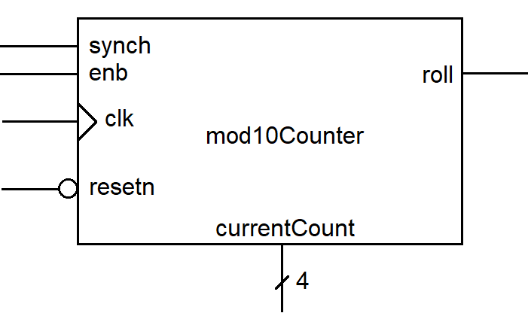
\includegraphics{image1.png}
\caption{The high-level interface for the mod 10 counter.}
\label{fig:mod10Symbol}
\end{figure}

Table~\ref{table:mod10StateTable} is the truth table for the currentCount output. When the
\textbf{enb} input is at logic 1, \textbf{currentCount} is incremented
mod 10 on the next positive clk edge. When the \textbf{synch} input
equals 1, \textbf{currentCount} goes to 4'b0000 on the next positive
\textbf{clk} edge. The \textbf{synch} input takes precedence over the
\textbf{enb} input, so if both are at logic 1 then \textbf{currentCount}
goes to 4'b0000 on the next positive \textbf{clk} edge.

\begin{longtable}[]{@{}
|  >{\raggedright\arraybackslash}p{(\columnwidth - 10\tabcolsep) * \real{0.1358}}|
  >{\raggedright\arraybackslash}p{(\columnwidth - 10\tabcolsep) * \real{0.1358}}|
  >{\raggedright\arraybackslash}p{(\columnwidth - 10\tabcolsep) * \real{0.1358}}|
  >{\raggedright\arraybackslash}p{(\columnwidth - 10\tabcolsep) * \real{0.1358}}|
  >{\raggedright\arraybackslash}p{(\columnwidth - 10\tabcolsep) * \real{0.2530}}|
  >{\raggedright\arraybackslash}p{(\columnwidth - 10\tabcolsep) * \real{0.2037}}|@{}}
\caption{The truth table for the currentCount output from the
mod10Counter.}\label{table:mod10StateTable}\tabularnewline
\toprule()
\begin{minipage}[b]{\linewidth}\raggedright
reset
\end{minipage} & \begin{minipage}[b]{\linewidth}\raggedright
clk
\end{minipage} & \begin{minipage}[b]{\linewidth}\raggedright
enb
\end{minipage} & \begin{minipage}[b]{\linewidth}\raggedright
synch
\end{minipage} & \begin{minipage}[b]{\linewidth}\raggedright
currentCount
\end{minipage} & \begin{minipage}[b]{\linewidth}\raggedright
Note
\end{minipage} \\
\midrule()
\endfirsthead
\toprule()
\begin{minipage}[b]{\linewidth}\raggedright
reset
\end{minipage} & \begin{minipage}[b]{\linewidth}\raggedright
clk
\end{minipage} & \begin{minipage}[b]{\linewidth}\raggedright
enb
\end{minipage} & \begin{minipage}[b]{\linewidth}\raggedright
synch
\end{minipage} & \begin{minipage}[b]{\linewidth}\raggedright
currentCount
\end{minipage} & \begin{minipage}[b]{\linewidth}\raggedright
Note
\end{minipage} \\
\midrule()
\endhead
0 & x & x & x & 0 & Asynch reset \\ \hline
1 & 0, 1, ↓ & x & x & currentCount & No clk edge \\ \hline
1 & ↑ & 0 & 0 & currentCount & Hold \\ \hline
1 & ↑ & 0 & 1 & 0 & Synch reset \\ \hline
1 & ↑ & 1 & 0 & (currentCount +1) mod 10 & Count up \\ \hline
1 & ↑ & 1 & 1 & 0 & Synch reset \\
\bottomrule()
\end{longtable}

Table~\ref{table:mod10Roll} is the truth table for the roll output. If \textbf{enb} is logic
1 when the \textbf{currentCount} equals 9, the \textbf{roll} output
equals logic 1. In all other cases the \textbf{roll} output should equal
logic 0. Note, the roll output does not depend on the \textbf{clk}, it's
a combinational logic block.

\begin{longtable}[]{@{}
| >{\raggedright\arraybackslash}p{(\columnwidth - 4\tabcolsep) * \real{0.2307}}|
  >{\raggedright\arraybackslash}p{(\columnwidth - 4\tabcolsep) * \real{0.5385}}|
  >{\raggedright\arraybackslash}p{(\columnwidth - 4\tabcolsep) * \real{0.2307}}|@{}}
\caption{The truth table for the roll output from the
mod10Counter.}\label{table:mod10Roll}\tabularnewline
\toprule()
\begin{minipage}[b]{\linewidth}\raggedright
enb
\end{minipage} & \begin{minipage}[b]{\linewidth}\raggedright
currentCount
\end{minipage} & \begin{minipage}[b]{\linewidth}\raggedright
roll
\end{minipage} \\
\midrule()
\endfirsthead
\toprule()
\begin{minipage}[b]{\linewidth}\raggedright
enb
\end{minipage} & \begin{minipage}[b]{\linewidth}\raggedright
currentCount
\end{minipage} & \begin{minipage}[b]{\linewidth}\raggedright
roll
\end{minipage} \\
\midrule()
\endhead
1 & currentCount \textless9 & 0 \\ \hline
1 & currentCount ==9 & 1 \\
\bottomrule()
\end{longtable}

Now that you have a solid grasp of how the mod10Counter should work,
let's turn our attention to how this is accomplished. The internal
organization of the mod10Counter is shown in Figure~\ref{fig:mod10sysArch}.

\begin{figure}
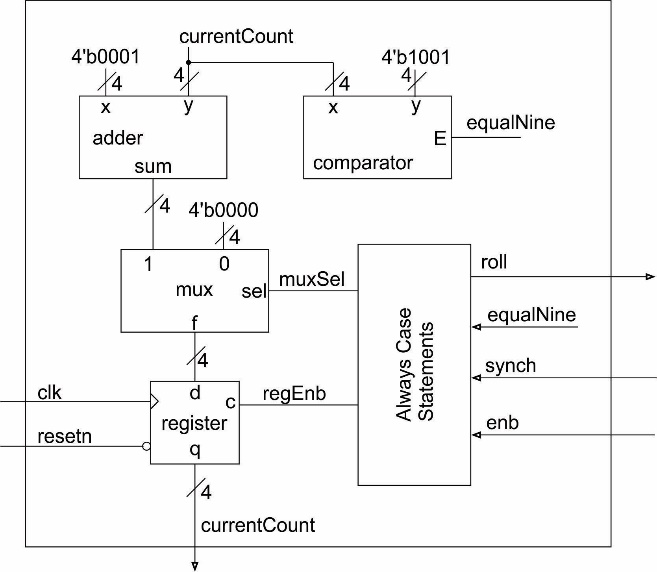
\includegraphics[width=0.6\paperwidth]{image2.jpeg}
\caption{The internal organization of the mod10counter module.}
\label{fig:mod10sysArch}
\end{figure}

You have been provided with the adder, comparator, mux, and register
shown in Figure~\ref{fig:mod10sysArch}. In addition to wiring these building blocks together,
you will need to define the logic inside the always/case block.

Use the truth tables in Table~\ref{table:mod10StateTable} and Table~\ref{table:mod10Roll} along with the hardware
organization in Figure~\ref{fig:mod10sysArch} to fill in Table~\ref{table:mod10alwaysCase} .



\begin{longtable}[]{@{}
| >{\raggedright\arraybackslash}p{(\columnwidth - 10\tabcolsep) * \real{0.1666}}|
  >{\raggedright\arraybackslash}p{(\columnwidth - 10\tabcolsep) * \real{0.1666}}|
  >{\raggedright\arraybackslash}p{(\columnwidth - 10\tabcolsep) * \real{0.1666}}|
  >{\raggedright\arraybackslash}p{(\columnwidth - 10\tabcolsep) * \real{0.1666}}|
  >{\raggedright\arraybackslash}p{(\columnwidth - 10\tabcolsep) * \real{0.1666}}|
  >{\raggedright\arraybackslash}p{(\columnwidth - 10\tabcolsep) * \real{0.1668}}|@{}}
\caption{The truth table for the always/case logic inside the mod10counter.}\label{table:mod10alwaysCase}\tabularnewline\toprule()
\begin{minipage}[b]{\linewidth}\raggedright
enb
\end{minipage} & \begin{minipage}[b]{\linewidth}\raggedright
synch
\end{minipage} & \begin{minipage}[b]{\linewidth}\raggedright
equalNine
\end{minipage} & \begin{minipage}[b]{\linewidth}\raggedright
muxSel
\end{minipage} & \begin{minipage}[b]{\linewidth}\raggedright
regEnb
\end{minipage} & \begin{minipage}[b]{\linewidth}\raggedright
roll
\end{minipage} \\
\midrule()
\endhead
0 & 0 & 0 & & & \\ \hline
0 & 0 & 1 & x & & \\ \hline
0 & 1 & 0 & & & \\ \hline
0 & 1 & 1 & & & \\ \hline
1 & 0 & 0 & & & 0 \\ \hline
1 & 0 & 1 & & 1 & \\ \hline
1 & 1 & 0 & & & \\ \hline
1 & 1 & 1 & & & \\
\bottomrule()
\end{longtable}

When you code your always/case statement, with a three-bit output and
then have three \emph{assign} statements that break this 3-bit output
into individual bits for muxSel, regEnb and roll.

You will need to demonstrate that your mod10counter operates correctly
by running the provided testbench. In order for you to verify correct
operation, you need to understand what output the simulation should
output so that you can compare that to what your simulation actually
producing. Any difference between these two indicate an error (either in
your understanding or circuit behavior) that need to be fixed. To do
this complete the timing diagram in Figure~\ref{fig:mod10TimingDiamgram} using the value from the
testbench.

\begin{landscape}
\begin{figure}
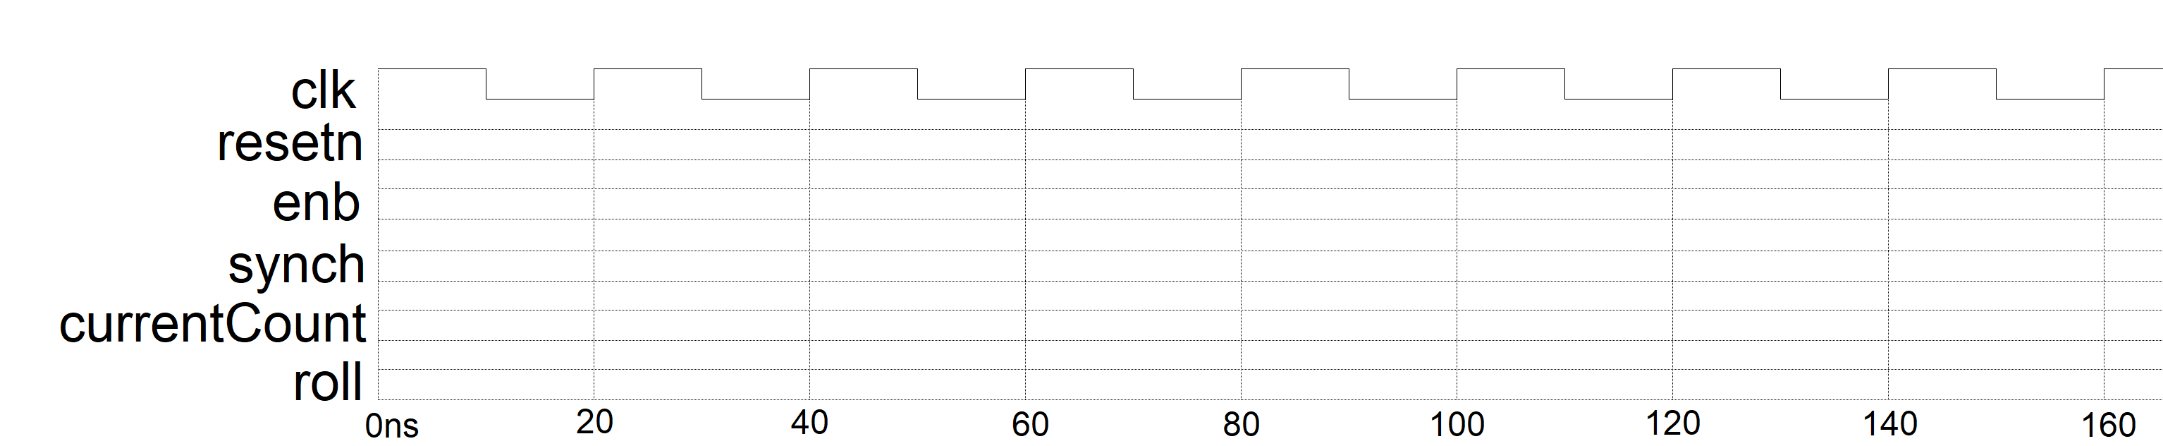
\includegraphics{image4.png}

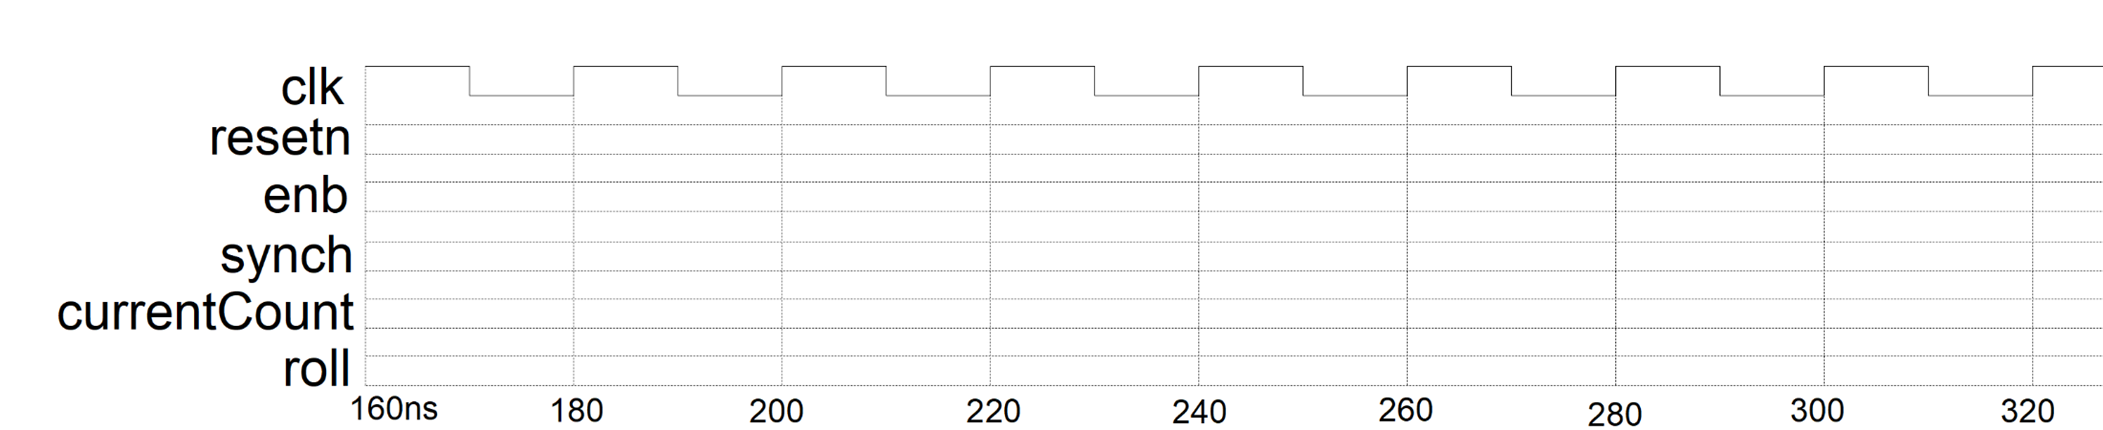
\includegraphics{image5.png}

\caption{A timing diagram for you to fill out based on the testbench
code for the mod10Counter. Note the diagram was too wide to be readable
in one line, so it has been broken in half at 160ns to make it easier to
you to read.}
\label{fig:mod10TimingDiamgram}
\end{figure}
\end{landscape}

\section{Do file}

You have been required to run simulation for almost every lab. The goal
of this requirement is not to just give you an extra task, but rather to
expeditated your debugging of your Verilog. However, if you have a lot
errors in your design, you may need to run the simulation multiple
times. Setting up all the signals, their colors and radix can be a time
consuming (and time wasting) task. The solution to this problem is to
create a script that sets up all the signals, their order, colors and
radixes. This script is called a do file.

Listing 1 shows a partial do file for the mod10counter testbench. The
``\#'' symbol is used to denote comments -- any text placed after them
is ignored by the do file interpreter.


\begin{lstlisting}[language=Verilog,
 caption={A partial do file for the mod10counter.},
basicstyle=\tiny\ttfamily,
 label={listing:hiLowWinVerilog},
 frame=single]
############################################
# Search Internet ``modelsim command reference manual''
############################################
vsim work.mod10counter_tb
restart -f
delete wave *

add wave -position end  sim:/mod10counter_tb/uut/clk
		<<you need more add waves here>>
add wave -position end  -radix unsigned -color greenyellow sim:/mod10counter_tb/uut/currentCount
 \end{lstlisting}
 
The first three lines start the simulation and delete any waveforms that
may be left over from a previous simulation. I included this in the do
file because I sometimes rerun a simulation to observe the modules
behavior at some earlier time.

The waveforms in the simulation are added using the ``add wave''
command. If you drag-and-drop a signal name into the waveform area, you
will see the add wave command appear in the console are at the bottom of
the ModelSim window. For example when I manually added the clk, I see:

\begin{verbatim}
add wave -position end sim:/mod10counter_tb/uut/clk
\end{verbatim}

I then add the color of the wave and the radix in between ``end'' and
``sim''. See Listing 1 for a couple of examples. You should use notepad
to edit the do file. Do NOT use a word processor like MS Word because
they tend to change the extensions of files when you save.

After editing the do file, it should be stored in the following folder:

\begin{verbatim}
<projectDirectory>\mod10Counter\simulation\modelsim
\end{verbatim}

Where \textless projectDirectory\textgreater{} is the path of your
project. If this folder does not exit, then you need to have to run
``Start Analysis and Elaboration'' at least once. You know you are in
the project directory when you see the project QPF file. You should run
the do file immediately after launching ModelSim from Quartus. You no
longer need to open the work directory and right mouse clicking on the
testbench file and select ``start simulation.'' Instead type:

\begin{verbatim}
do mod10counter_tbWaveSetup.do
\end{verbatim}

When you run the do file, you should see something similar to Figure~\ref{fig:mod10console}.

\begin{figure}
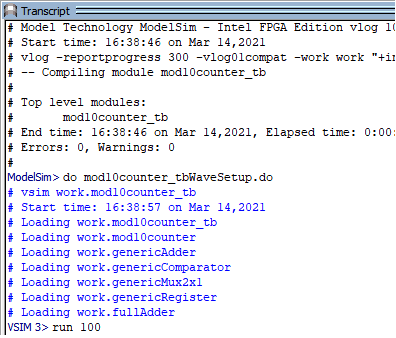
\includegraphics[width=0.4\paperwidth]{image6.png}
\caption{The console output when the mod10counter do file is run.}
\label{fig:mod10console}
\end{figure}

The ModelSim console allows tab completion, a feature that helps you
fill-in the characters of long file name. To use tab completion, type
the first few characters of a command/filename and then press Tab. If
there are no other file names that match what you have typed in, the
remainder of the file name will be auto-complete for you. If there is
more than one filename choice, the command/filename will be completed up
to the ambiguity and the console will provide a list of candidate
filenames.

You can issue a variety of commands in the console window. On of my
favorite is ``run \textless time\textgreater'' to simulate some amount
of time. I found this VERY handy when debugging my Verilog code.

\section{Testbench}

Edit the do file provided on Canvas to produce the following output.

\begin{tabular}{p{3cm}p{3cm}p{3cm}}
  clk 		& default 		& green trace \\ 
  reset 	& default 		& green trace \\ 
  enb 		& default 		& gold trace \\ 
  synch 	& default 		& gold trace \\ 
  roll 		& default 		& yellow trace \\ 
  currentCount 	& unsigned & greenyellow trace \\ 
\end{tabular}

You need to look at the values produced by the mod10counter and compare
them against the values in Table~\ref{table:mod10StateTable}. Look for discrepancies
starting at time 0 and only advancing the simulation when everything is
correct. You will have to transcend the design hierarchy to find the
source of your errors. Most of my errors are due to incorrect wiring or
modules -- wrong names or wrong signal order.


\section{Turn in}

You may work in teams of at most two. Make a record of your response to
the items below and turn them in a single copy as your team's solution
on Canvas using the instructions posted there. Include the names of both
team members at the top of your solutions. Use complete English
sentences to introduce what each of the following listed items (below)
is and how it was derived. In addition to this submission, you will be
expected to demonstrate your circuit at the beginning of your lab
section next week.

\subsubsection{Mod10 Counter Verilog}

\begin{itemize}
\item
  Complete Table~\ref{table:mod10alwaysCase} and Figure~\ref{fig:mod10TimingDiamgram}.
\item
  Verilog code for the body of the mode10counter module (courier 8-point
  font single spaced), leave out header comments.
\item
  Timing diagram of the mod10counter using do file in the testbench.
\item
  Do file.
\end{itemize}

